\documentclass[1p]{elsarticle_modified}
%\bibliographystyle{elsarticle-num}

%\usepackage[colorlinks]{hyperref}
%\usepackage{abbrmath_seonhwa} %\Abb, \Ascr, \Acal ,\Abf, \Afrak
\usepackage{amsfonts}
\usepackage{amssymb}
\usepackage{amsmath}
\usepackage{amsthm}
\usepackage{scalefnt}
\usepackage{amsbsy}
\usepackage{kotex}
\usepackage{caption}
\usepackage{subfig}
\usepackage{color}
\usepackage{graphicx}
\usepackage{xcolor} %% white, black, red, green, blue, cyan, magenta, yellow
\usepackage{float}
\usepackage{setspace}
\usepackage{hyperref}

\usepackage{tikz}
\usetikzlibrary{arrows}

\usepackage{multirow}
\usepackage{array} % fixed length table
\usepackage{hhline}

%%%%%%%%%%%%%%%%%%%%%
\makeatletter
\renewcommand*\env@matrix[1][\arraystretch]{%
	\edef\arraystretch{#1}%
	\hskip -\arraycolsep
	\let\@ifnextchar\new@ifnextchar
	\array{*\c@MaxMatrixCols c}}
\makeatother %https://tex.stackexchange.com/questions/14071/how-can-i-increase-the-line-spacing-in-a-matrix
%%%%%%%%%%%%%%%

\usepackage[normalem]{ulem}

\newcommand{\msout}[1]{\ifmmode\text{\sout{\ensuremath{#1}}}\else\sout{#1}\fi}
%SOURCE: \msout is \stkout macro in https://tex.stackexchange.com/questions/20609/strikeout-in-math-mode

\newcommand{\cancel}[1]{
	\ifmmode
	{\color{red}\msout{#1}}
	\else
	{\color{red}\sout{#1}}
	\fi
}

\newcommand{\add}[1]{
	{\color{blue}\uwave{#1}}
}

\newcommand{\replace}[2]{
	\ifmmode
	{\color{red}\msout{#1}}{\color{blue}\uwave{#2}}
	\else
	{\color{red}\sout{#1}}{\color{blue}\uwave{#2}}
	\fi
}

\newcommand{\Sol}{\mathcal{S}} %segment
\newcommand{\D}{D} %diagram
\newcommand{\A}{\mathcal{A}} %arc


%%%%%%%%%%%%%%%%%%%%%%%%%%%%%5 test

\def\sl{\operatorname{\textup{SL}}(2,\Cbb)}
\def\psl{\operatorname{\textup{PSL}}(2,\Cbb)}
\def\quan{\mkern 1mu \triangleright \mkern 1mu}

\theoremstyle{definition}
\newtheorem{thm}{Theorem}[section]
\newtheorem{prop}[thm]{Proposition}
\newtheorem{lem}[thm]{Lemma}
\newtheorem{ques}[thm]{Question}
\newtheorem{cor}[thm]{Corollary}
\newtheorem{defn}[thm]{Definition}
\newtheorem{exam}[thm]{Example}
\newtheorem{rmk}[thm]{Remark}
\newtheorem{alg}[thm]{Algorithm}

\newcommand{\I}{\sqrt{-1}}
\begin{document}

%\begin{frontmatter}
%
%\title{Boundary parabolic representations of knots up to 8 crossings}
%
%%% Group authors per affiliation:
%\author{Yunhi Cho} 
%\address{Department of Mathematics, University of Seoul, Seoul, Korea}
%\ead{yhcho@uos.ac.kr}
%
%
%\author{Seonhwa Kim} %\fnref{s_kim}}
%\address{Center for Geometry and Physics, Institute for Basic Science, Pohang, 37673, Korea}
%\ead{ryeona17@ibs.re.kr}
%
%\author{Hyuk Kim}
%\address{Department of Mathematical Sciences, Seoul National University, Seoul 08826, Korea}
%\ead{hyukkim@snu.ac.kr}
%
%\author{Seokbeom Yoon}
%\address{Department of Mathematical Sciences, Seoul National University, Seoul, 08826,  Korea}
%\ead{sbyoon15@snu.ac.kr}
%
%\begin{abstract}
%We find all boundary parabolic representation of knots up to 8 crossings.
%
%\end{abstract}
%\begin{keyword}
%    \MSC[2010] 57M25 
%\end{keyword}
%
%\end{frontmatter}

%\linenumbers
%\tableofcontents
%
\newcommand\colored[1]{\textcolor{white}{\rule[-0.35ex]{0.8em}{1.4ex}}\kern-0.8em\color{red} #1}%
%\newcommand\colored[1]{\textcolor{white}{ #1}\kern-2.17ex	\textcolor{white}{ #1}\kern-1.81ex	\textcolor{white}{ #1}\kern-2.15ex\color{red}#1	}

{\Large $\underline{11n_{145}~(K11n_{145})}$}

\setlength{\tabcolsep}{10pt}
\renewcommand{\arraystretch}{1.6}
\vspace{1cm}\begin{tabular}{m{100pt}>{\centering\arraybackslash}m{274pt}}
\multirow{5}{120pt}{
	\centering
	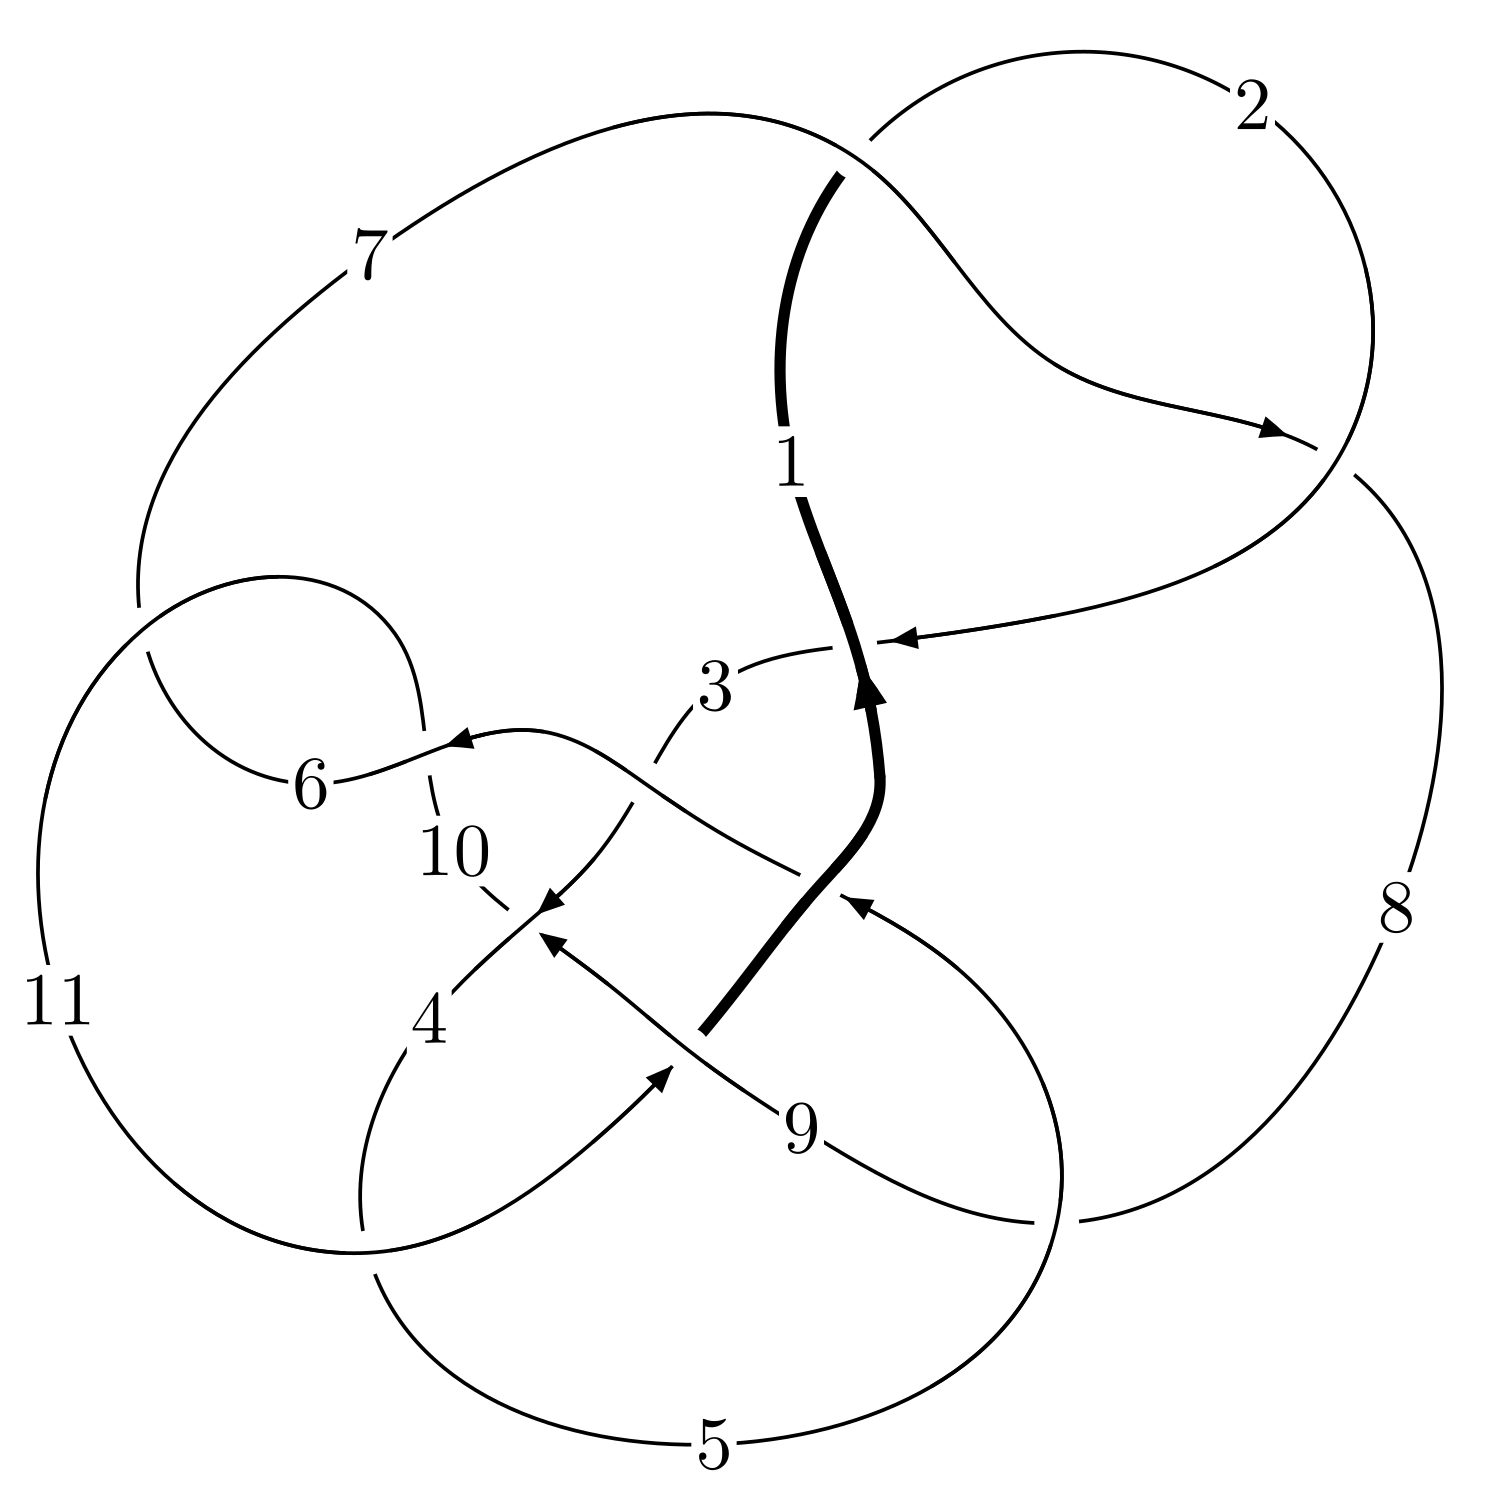
\includegraphics[width=112pt]{../../../GIT/diagram.site/Diagrams/png/761_11n_145.png}\\
\ \ \ A knot diagram\footnotemark}&
\allowdisplaybreaks
\textbf{Linearized knot diagam} \\
\cline{2-2}
 &
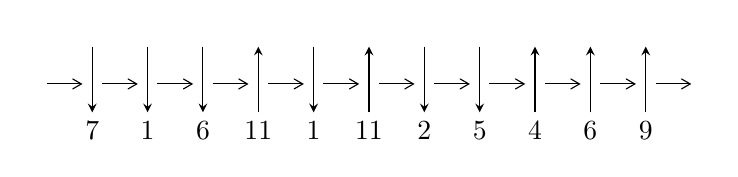
\begin{tikzpicture}[x=20pt, y=17pt]
	% nodes
	\node (C0) at (0, 0) {};
	\node (C1) at (1, 0) {};
	\node (C1U) at (1, +1) {};
	\node (C1D) at (1, -1) {7};

	\node (C2) at (2, 0) {};
	\node (C2U) at (2, +1) {};
	\node (C2D) at (2, -1) {1};

	\node (C3) at (3, 0) {};
	\node (C3U) at (3, +1) {};
	\node (C3D) at (3, -1) {6};

	\node (C4) at (4, 0) {};
	\node (C4U) at (4, +1) {};
	\node (C4D) at (4, -1) {11};

	\node (C5) at (5, 0) {};
	\node (C5U) at (5, +1) {};
	\node (C5D) at (5, -1) {1};

	\node (C6) at (6, 0) {};
	\node (C6U) at (6, +1) {};
	\node (C6D) at (6, -1) {11};

	\node (C7) at (7, 0) {};
	\node (C7U) at (7, +1) {};
	\node (C7D) at (7, -1) {2};

	\node (C8) at (8, 0) {};
	\node (C8U) at (8, +1) {};
	\node (C8D) at (8, -1) {5};

	\node (C9) at (9, 0) {};
	\node (C9U) at (9, +1) {};
	\node (C9D) at (9, -1) {4};

	\node (C10) at (10, 0) {};
	\node (C10U) at (10, +1) {};
	\node (C10D) at (10, -1) {6};

	\node (C11) at (11, 0) {};
	\node (C11U) at (11, +1) {};
	\node (C11D) at (11, -1) {9};
	\node (C12) at (12, 0) {};

	% arrows
	\draw[->,>={angle 60}]
	(C0) edge (C1) (C1) edge (C2) (C2) edge (C3) (C3) edge (C4) (C4) edge (C5) (C5) edge (C6) (C6) edge (C7) (C7) edge (C8) (C8) edge (C9) (C9) edge (C10) (C10) edge (C11) (C11) edge (C12) ;	\draw[->,>=stealth]
	(C1U) edge (C1D) (C2U) edge (C2D) (C3U) edge (C3D) (C4D) edge (C4U) (C5U) edge (C5D) (C6D) edge (C6U) (C7U) edge (C7D) (C8U) edge (C8D) (C9D) edge (C9U) (C10D) edge (C10U) (C11D) edge (C11U) ;
	\end{tikzpicture} \\
\hhline{~~} \\& 
\textbf{Solving Sequence} \\ \cline{2-2} 
 &
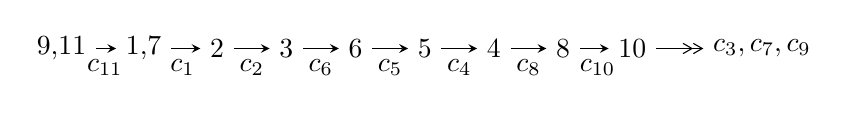
\begin{tikzpicture}[x=25pt, y=7pt]
	% node
	\node (A0) at (-1/8, 0) {9,11};
	\node (A1) at (17/16, 0) {1,7};
	\node (A2) at (17/8, 0) {2};
	\node (A3) at (25/8, 0) {3};
	\node (A4) at (33/8, 0) {6};
	\node (A5) at (41/8, 0) {5};
	\node (A6) at (49/8, 0) {4};
	\node (A7) at (57/8, 0) {8};
	\node (A8) at (65/8, 0) {10};
	\node (C1) at (1/2, -1) {$c_{11}$};
	\node (C2) at (13/8, -1) {$c_{1}$};
	\node (C3) at (21/8, -1) {$c_{2}$};
	\node (C4) at (29/8, -1) {$c_{6}$};
	\node (C5) at (37/8, -1) {$c_{5}$};
	\node (C6) at (45/8, -1) {$c_{4}$};
	\node (C7) at (53/8, -1) {$c_{8}$};
	\node (C8) at (61/8, -1) {$c_{10}$};
	\node (A9) at (10, 0) {$c_{3},c_{7},c_{9}$};

	% edge
	\draw[->,>=stealth]	
	(A0) edge (A1) (A1) edge (A2) (A2) edge (A3) (A3) edge (A4) (A4) edge (A5) (A5) edge (A6) (A6) edge (A7) (A7) edge (A8) ;
	\draw[->>,>={angle 60}]	
	(A8) edge (A9);
\end{tikzpicture} \\ 

\end{tabular} \\

\footnotetext{
The image of knot diagram is generated by the software ``\textbf{Draw programme}" developed by Andrew Bartholomew(\url{http://www.layer8.co.uk/maths/draw/index.htm\#Running-draw}), where we modified some parts for our purpose(\url{https://github.com/CATsTAILs/LinksPainter}).
}\phantom \\ \newline 
\centering \textbf{Ideals for irreducible components\footnotemark of $X_{\text{par}}$} 
 
\begin{align*}
I^u_{1}&=\langle 
u^{11}+u^{10}+2 u^9+u^8+4 u^7+2 u^6+3 u^5- u^4+u^3+2 u^2+b+2 u+1,\\
\phantom{I^u_{1}}&\phantom{= \langle  }3 u^{11}+5 u^{10}+6 u^9+3 u^8+12 u^7+11 u^6+6 u^5-6 u^4+5 u^3+8 u^2+a+8 u+2,\\
\phantom{I^u_{1}}&\phantom{= \langle  }u^{12}+2 u^{11}+3 u^{10}+2 u^9+5 u^8+5 u^7+5 u^6- u^5+2 u^4+2 u^3+5 u^2+2 u+1\rangle \\
I^u_{2}&=\langle 
u^6-2 u^5+2 u^4+b- u+1,\;-2 u^7+6 u^6-9 u^5+5 u^4-2 u^3+4 u^2+a-7 u+2,\\
\phantom{I^u_{2}}&\phantom{= \langle  }u^8-3 u^7+5 u^6-4 u^5+3 u^4-3 u^3+4 u^2-2 u+1\rangle \\
\\
\end{align*}
\raggedright * 2 irreducible components of $\dim_{\mathbb{C}}=0$, with total 20 representations.\\
\footnotetext{All coefficients of polynomials are rational numbers. But the coefficients are sometimes approximated in decimal forms when there is not enough margin.}
\newpage
\renewcommand{\arraystretch}{1}
\centering \section*{I. $I^u_{1}= \langle u^{11}+u^{10}+\cdots+b+1,\;3 u^{11}+5 u^{10}+\cdots+a+2,\;u^{12}+2 u^{11}+\cdots+2 u+1 \rangle$}
\flushleft \textbf{(i) Arc colorings}\\
\begin{tabular}{m{7pt} m{180pt} m{7pt} m{180pt} }
\flushright $a_{9}=$&$\begin{pmatrix}0\\u\end{pmatrix}$ \\
\flushright $a_{11}=$&$\begin{pmatrix}1\\0\end{pmatrix}$ \\
\flushright $a_{1}=$&$\begin{pmatrix}1\\- u^2\end{pmatrix}$ \\
\flushright $a_{7}=$&$\begin{pmatrix}-3 u^{11}-5 u^{10}+\cdots-8 u-2\\- u^{11}- u^{10}-2 u^9- u^8-4 u^7-2 u^6-3 u^5+u^4- u^3-2 u^2-2 u-1\end{pmatrix}$ \\
\flushright $a_{2}=$&$\begin{pmatrix}-2 u^{11}-3 u^{10}+\cdots-2 u-1\\- u^{11}- u^9-3 u^7+u^6- u^5+u^4- u^3-2 u^2\end{pmatrix}$ \\
\flushright $a_{3}=$&$\begin{pmatrix}-2 u^{11}-2 u^{10}-3 u^9-8 u^7-3 u^6-3 u^5+6 u^4-7 u^3-3 u^2-2 u\\u^{11}+u^{10}+2 u^9+u^8+4 u^7+2 u^6+3 u^5- u^4+u^3+2 u^2+2 u+1\end{pmatrix}$ \\
\flushright $a_{6}=$&$\begin{pmatrix}-2 u^{11}-4 u^{10}+\cdots-6 u-1\\- u^{11}- u^{10}-2 u^9- u^8-4 u^7-2 u^6-3 u^5+u^4- u^3-2 u^2-2 u-1\end{pmatrix}$ \\
\flushright $a_{5}=$&$\begin{pmatrix}- u^{11}-3 u^{10}-4 u^9-2 u^8-5 u^7-8 u^6-6 u^5+4 u^4- u^3-5 u^2-6 u-2\\-2 u^{10}-2 u^9-2 u^8- u^7-7 u^6-3 u^5+2 u^3-4 u^2-3 u-2\end{pmatrix}$ \\
\flushright $a_{4}=$&$\begin{pmatrix}- u^{11}- u^{10}-2 u^9-4 u^7- u^6-3 u^5+4 u^4-3 u^3- u^2-3 u\\-2 u^{10}-2 u^9-2 u^8- u^7-7 u^6-3 u^5+2 u^3-4 u^2-3 u-2\end{pmatrix}$ \\
\flushright $a_{8}=$&$\begin{pmatrix}u^{11}+2 u^{10}+2 u^9+2 u^8+3 u^7+6 u^6+u^5- u^3+6 u^2+u+2\\u^{11}+u^{10}+2 u^9+u^8+3 u^7+3 u^6+2 u^5- u^4+4 u^2+2 u+1\end{pmatrix}$ \\
\flushright $a_{10}=$&$\begin{pmatrix}- u^{11}- u^{10}- u^9- u^8-3 u^7-2 u^6- u^3-2 u^2- u\\u^{11}+2 u^{10}+u^9+2 u^8+3 u^7+5 u^6- u^5+u^4+4 u^2+2 u+1\end{pmatrix}$\\ \flushright $a_{10}=$&$\begin{pmatrix}- u^{11}- u^{10}- u^9- u^8-3 u^7-2 u^6- u^3-2 u^2- u\\u^{11}+2 u^{10}+u^9+2 u^8+3 u^7+5 u^6- u^5+u^4+4 u^2+2 u+1\end{pmatrix}$\\&\end{tabular}
\flushleft \textbf{(ii) Obstruction class $= -1$}\\~\\
\flushleft \textbf{(iii) Cusp Shapes $= -3 u^{11}-7 u^{10}-8 u^9-7 u^8-14 u^7-21 u^6-8 u^5- u^3-16 u^2-4 u-9$}\\~\\
\newpage\renewcommand{\arraystretch}{1}
\flushleft \textbf{(iv) u-Polynomials at the component}\newline \\
\begin{tabular}{m{50pt}|m{274pt}}
Crossings & \hspace{64pt}u-Polynomials at each crossing \\
\hline $$\begin{aligned}c_{1},c_{7}\end{aligned}$$&$\begin{aligned}
&u^{12}-11 u^{11}+\cdots-48 u+16
\end{aligned}$\\
\hline $$\begin{aligned}c_{2}\end{aligned}$$&$\begin{aligned}
&u^{12}+9 u^{11}+\cdots+896 u+256
\end{aligned}$\\
\hline $$\begin{aligned}c_{3}\end{aligned}$$&$\begin{aligned}
&u^{12}-4 u^{11}+\cdots-4 u+1
\end{aligned}$\\
\hline $$\begin{aligned}c_{4}\end{aligned}$$&$\begin{aligned}
&u^{12}- u^{11}+\cdots+4 u+10
\end{aligned}$\\
\hline $$\begin{aligned}c_{5},c_{8}\end{aligned}$$&$\begin{aligned}
&u^{12}+2 u^{11}+\cdots-16 u^2+1
\end{aligned}$\\
\hline $$\begin{aligned}c_{6},c_{9},c_{10}\end{aligned}$$&$\begin{aligned}
&u^{12}-10 u^{10}+\cdots- u+1
\end{aligned}$\\
\hline $$\begin{aligned}c_{11}\end{aligned}$$&$\begin{aligned}
&u^{12}+2 u^{11}+\cdots+2 u+1
\end{aligned}$\\
\hline
\end{tabular}\\~\\
\newpage\renewcommand{\arraystretch}{1}
\flushleft \textbf{(v) Riley Polynomials at the component}\newline \\
\begin{tabular}{m{50pt}|m{274pt}}
Crossings & \hspace{64pt}Riley Polynomials at each crossing \\
\hline $$\begin{aligned}c_{1},c_{7}\end{aligned}$$&$\begin{aligned}
&y^{12}-9 y^{11}+\cdots-896 y+256
\end{aligned}$\\
\hline $$\begin{aligned}c_{2}\end{aligned}$$&$\begin{aligned}
&y^{12}+59 y^{11}+\cdots+253952 y+65536
\end{aligned}$\\
\hline $$\begin{aligned}c_{3}\end{aligned}$$&$\begin{aligned}
&y^{12}-30 y^{11}+\cdots-16 y+1
\end{aligned}$\\
\hline $$\begin{aligned}c_{4}\end{aligned}$$&$\begin{aligned}
&y^{12}-25 y^{11}+\cdots-896 y+100
\end{aligned}$\\
\hline $$\begin{aligned}c_{5},c_{8}\end{aligned}$$&$\begin{aligned}
&y^{12}+26 y^{11}+\cdots-32 y+1
\end{aligned}$\\
\hline $$\begin{aligned}c_{6},c_{9},c_{10}\end{aligned}$$&$\begin{aligned}
&y^{12}-20 y^{11}+\cdots+3 y+1
\end{aligned}$\\
\hline $$\begin{aligned}c_{11}\end{aligned}$$&$\begin{aligned}
&y^{12}+2 y^{11}+\cdots+6 y+1
\end{aligned}$\\
\hline
\end{tabular}\\~\\
\newpage\flushleft \textbf{(vi) Complex Volumes and Cusp Shapes}
$$\begin{array}{c|c|c}  
\text{Solutions to }I^u_{1}& \I (\text{vol} + \sqrt{-1}CS) & \text{Cusp shape}\\
 \hline 
\begin{aligned}
u &= \phantom{-}0.800801 + 0.482482 I \\
a &= \phantom{-}0.183380 + 0.498565 I \\
b &= \phantom{-}0.698671 + 0.235425 I\end{aligned}
 & \phantom{-}1.43652 + 0.62326 I & \phantom{-}4.44877 + 0.65496 I \\ \hline\begin{aligned}
u &= \phantom{-}0.800801 - 0.482482 I \\
a &= \phantom{-}0.183380 - 0.498565 I \\
b &= \phantom{-}0.698671 - 0.235425 I\end{aligned}
 & \phantom{-}1.43652 - 0.62326 I & \phantom{-}4.44877 - 0.65496 I \\ \hline\begin{aligned}
u &= -0.372107 + 0.751953 I \\
a &= -0.81363 + 1.82447 I \\
b &= \phantom{-}0.243009 + 0.355918 I\end{aligned}
 & -9.07675 - 1.52290 I & -4.89097 + 7.64925 I \\ \hline\begin{aligned}
u &= -0.372107 - 0.751953 I \\
a &= -0.81363 - 1.82447 I \\
b &= \phantom{-}0.243009 - 0.355918 I\end{aligned}
 & -9.07675 + 1.52290 I & -4.89097 - 7.64925 I \\ \hline\begin{aligned}
u &= \phantom{-}0.690074 + 1.109750 I \\
a &= -0.458254 - 0.957045 I \\
b &= -0.715998 - 0.535824 I\end{aligned}
 & -0.63619 + 5.03255 I & -5.39872 - 6.82429 I \\ \hline\begin{aligned}
u &= \phantom{-}0.690074 - 1.109750 I \\
a &= -0.458254 + 0.957045 I \\
b &= -0.715998 + 0.535824 I\end{aligned}
 & -0.63619 - 5.03255 I & -5.39872 + 6.82429 I \\ \hline\begin{aligned}
u &= -0.981759 + 0.915783 I \\
a &= \phantom{-}1.31213 - 0.66172 I \\
b &= \phantom{-}2.49508 + 1.02200 I\end{aligned}
 & \phantom{-}11.48080 + 2.02735 I & -0.446845 + 0.080322 I \\ \hline\begin{aligned}
u &= -0.981759 - 0.915783 I \\
a &= \phantom{-}1.31213 + 0.66172 I \\
b &= \phantom{-}2.49508 - 1.02200 I\end{aligned}
 & \phantom{-}11.48080 - 2.02735 I & -0.446845 - 0.080322 I \\ \hline\begin{aligned}
u &= -0.924436 + 1.006840 I \\
a &= -0.21708 + 2.14841 I \\
b &= -2.45017 + 1.30392 I\end{aligned}
 & \phantom{-}11.1731 - 9.0121 I & -0.90831 + 4.12550 I \\ \hline\begin{aligned}
u &= -0.924436 - 1.006840 I \\
a &= -0.21708 - 2.14841 I \\
b &= -2.45017 - 1.30392 I\end{aligned}
 & \phantom{-}11.1731 + 9.0121 I & -0.90831 - 4.12550 I\\
 \hline 
 \end{array}$$\newpage$$\begin{array}{c|c|c}  
\text{Solutions to }I^u_{1}& \I (\text{vol} + \sqrt{-1}CS) & \text{Cusp shape}\\
 \hline 
\begin{aligned}
u &= -0.212573 + 0.487267 I \\
a &= \phantom{-}0.49344 - 1.36791 I \\
b &= -0.270602 - 0.384607 I\end{aligned}
 & -1.218070 - 0.691278 I & -5.30392 + 1.72582 I \\ \hline\begin{aligned}
u &= -0.212573 - 0.487267 I \\
a &= \phantom{-}0.49344 + 1.36791 I \\
b &= -0.270602 + 0.384607 I\end{aligned}
 & -1.218070 + 0.691278 I & -5.30392 - 1.72582 I\\
 \hline 
 \end{array}$$\newpage\newpage\renewcommand{\arraystretch}{1}
\centering \section*{II. $I^u_{2}= \langle u^6-2 u^5+2 u^4+b- u+1,\;-2 u^7+6 u^6+\cdots+a+2,\;u^8-3 u^7+\cdots-2 u+1 \rangle$}
\flushleft \textbf{(i) Arc colorings}\\
\begin{tabular}{m{7pt} m{180pt} m{7pt} m{180pt} }
\flushright $a_{9}=$&$\begin{pmatrix}0\\u\end{pmatrix}$ \\
\flushright $a_{11}=$&$\begin{pmatrix}1\\0\end{pmatrix}$ \\
\flushright $a_{1}=$&$\begin{pmatrix}1\\- u^2\end{pmatrix}$ \\
\flushright $a_{7}=$&$\begin{pmatrix}2 u^7-6 u^6+9 u^5-5 u^4+2 u^3-4 u^2+7 u-2\\- u^6+2 u^5-2 u^4+u-1\end{pmatrix}$ \\
\flushright $a_{2}=$&$\begin{pmatrix}-4 u^7+11 u^6-16 u^5+9 u^4-5 u^3+8 u^2-12 u+4\\- u^7+3 u^6-5 u^5+4 u^4-2 u^3+u^2-3 u+2\end{pmatrix}$ \\
\flushright $a_{3}=$&$\begin{pmatrix}-4 u^7+10 u^6-14 u^5+6 u^4-4 u^3+7 u^2-11 u+1\\u^6-2 u^5+2 u^4- u+1\end{pmatrix}$ \\
\flushright $a_{6}=$&$\begin{pmatrix}2 u^7-5 u^6+7 u^5-3 u^4+2 u^3-4 u^2+6 u-1\\- u^6+2 u^5-2 u^4+u-1\end{pmatrix}$ \\
\flushright $a_{5}=$&$\begin{pmatrix}2 u^7-6 u^6+9 u^5-6 u^4+3 u^3-5 u^2+7 u-3\\u^7-3 u^6+5 u^5-4 u^4+2 u^3-2 u^2+3 u-2\end{pmatrix}$ \\
\flushright $a_{4}=$&$\begin{pmatrix}u^7-3 u^6+4 u^5-2 u^4+u^3-3 u^2+4 u-1\\u^7-3 u^6+5 u^5-4 u^4+2 u^3-2 u^2+3 u-2\end{pmatrix}$ \\
\flushright $a_{8}=$&$\begin{pmatrix}-3 u^7+9 u^6-14 u^5+9 u^4-5 u^3+7 u^2-11 u+3\\- u^7+4 u^6-7 u^5+6 u^4-3 u^3+4 u^2-5 u+3\end{pmatrix}$ \\
\flushright $a_{10}=$&$\begin{pmatrix}- u^7+2 u^6-2 u^5- u^4+u^3- u-1\\- u^7+3 u^6-5 u^5+4 u^4-3 u^3+3 u^2-3 u+1\end{pmatrix}$\\ \flushright $a_{10}=$&$\begin{pmatrix}- u^7+2 u^6-2 u^5- u^4+u^3- u-1\\- u^7+3 u^6-5 u^5+4 u^4-3 u^3+3 u^2-3 u+1\end{pmatrix}$\\&\end{tabular}
\flushleft \textbf{(ii) Obstruction class $= 1$}\\~\\
\flushleft \textbf{(iii) Cusp Shapes $= -2 u^7+5 u^5-11 u^4+2 u^3-4 u^2+7 u-9$}\\~\\
\newpage\renewcommand{\arraystretch}{1}
\flushleft \textbf{(iv) u-Polynomials at the component}\newline \\
\begin{tabular}{m{50pt}|m{274pt}}
Crossings & \hspace{64pt}u-Polynomials at each crossing \\
\hline $$\begin{aligned}c_{1}\end{aligned}$$&$\begin{aligned}
&u^8+u^7-4 u^6-2 u^5+7 u^4+u^3-5 u^2+2
\end{aligned}$\\
\hline $$\begin{aligned}c_{2}\end{aligned}$$&$\begin{aligned}
&u^8+9 u^7+34 u^6+72 u^5+97 u^4+87 u^3+53 u^2+20 u+4
\end{aligned}$\\
\hline $$\begin{aligned}c_{3}\end{aligned}$$&$\begin{aligned}
&u^8-9 u^7+31 u^6-51 u^5+42 u^4-20 u^3+9 u^2-2 u+1
\end{aligned}$\\
\hline $$\begin{aligned}c_{4}\end{aligned}$$&$\begin{aligned}
&u^8+u^6+2 u^5+3 u^4+3 u^3- u^2+2
\end{aligned}$\\
\hline $$\begin{aligned}c_{5},c_{8}\end{aligned}$$&$\begin{aligned}
&u^8- u^7- u^6- u^5+2 u^4+2 u^3+3 u^2+2 u+1
\end{aligned}$\\
\hline $$\begin{aligned}c_{6},c_{9}\end{aligned}$$&$\begin{aligned}
&u^8- u^7+2 u^6- u^5- u^4+3 u^3- u^2- u+1
\end{aligned}$\\
\hline $$\begin{aligned}c_{7}\end{aligned}$$&$\begin{aligned}
&u^8- u^7-4 u^6+2 u^5+7 u^4- u^3-5 u^2+2
\end{aligned}$\\
\hline $$\begin{aligned}c_{10}\end{aligned}$$&$\begin{aligned}
&u^8+u^7+2 u^6+u^5- u^4-3 u^3- u^2+u+1
\end{aligned}$\\
\hline $$\begin{aligned}c_{11}\end{aligned}$$&$\begin{aligned}
&u^8-3 u^7+5 u^6-4 u^5+3 u^4-3 u^3+4 u^2-2 u+1
\end{aligned}$\\
\hline
\end{tabular}\\~\\
\newpage\renewcommand{\arraystretch}{1}
\flushleft \textbf{(v) Riley Polynomials at the component}\newline \\
\begin{tabular}{m{50pt}|m{274pt}}
Crossings & \hspace{64pt}Riley Polynomials at each crossing \\
\hline $$\begin{aligned}c_{1},c_{7}\end{aligned}$$&$\begin{aligned}
&y^8-9 y^7+34 y^6-72 y^5+97 y^4-87 y^3+53 y^2-20 y+4
\end{aligned}$\\
\hline $$\begin{aligned}c_{2}\end{aligned}$$&$\begin{aligned}
&y^8-13 y^7+54 y^6-48 y^5+133 y^4+105 y^3+105 y^2+24 y+16
\end{aligned}$\\
\hline $$\begin{aligned}c_{3}\end{aligned}$$&$\begin{aligned}
&y^8-19 y^7+127 y^6-339 y^5+248 y^4+214 y^3+85 y^2+14 y+1
\end{aligned}$\\
\hline $$\begin{aligned}c_{4}\end{aligned}$$&$\begin{aligned}
&y^8+2 y^7+7 y^6- y^4-11 y^3+13 y^2-4 y+4
\end{aligned}$\\
\hline $$\begin{aligned}c_{5},c_{8}\end{aligned}$$&$\begin{aligned}
&y^8-3 y^7+3 y^6+5 y^5+8 y^4+10 y^3+5 y^2+2 y+1
\end{aligned}$\\
\hline $$\begin{aligned}c_{6},c_{9},c_{10}\end{aligned}$$&$\begin{aligned}
&y^8+3 y^7- y^5+3 y^4-5 y^3+5 y^2-3 y+1
\end{aligned}$\\
\hline $$\begin{aligned}c_{11}\end{aligned}$$&$\begin{aligned}
&y^8+y^7+7 y^6+4 y^5+15 y^4+9 y^3+10 y^2+4 y+1
\end{aligned}$\\
\hline
\end{tabular}\\~\\
\newpage\flushleft \textbf{(vi) Complex Volumes and Cusp Shapes}
$$\begin{array}{c|c|c}  
\text{Solutions to }I^u_{2}& \I (\text{vol} + \sqrt{-1}CS) & \text{Cusp shape}\\
 \hline 
\begin{aligned}
u &= -0.601219 + 0.700245 I \\
a &= -1.25463 - 1.13763 I \\
b &= \phantom{-}0.04009 - 1.51942 I\end{aligned}
 & -5.61184 - 2.16662 I & -1.31720 + 3.92427 I \\ \hline\begin{aligned}
u &= -0.601219 - 0.700245 I \\
a &= -1.25463 + 1.13763 I \\
b &= \phantom{-}0.04009 + 1.51942 I\end{aligned}
 & -5.61184 + 2.16662 I & -1.31720 - 3.92427 I \\ \hline\begin{aligned}
u &= \phantom{-}0.975658 + 0.743632 I \\
a &= \phantom{-}0.205573 + 0.088262 I \\
b &= \phantom{-}0.804982 + 0.154967 I\end{aligned}
 & \phantom{-}1.42321 + 1.81732 I & \phantom{-}3.74465 - 3.23500 I \\ \hline\begin{aligned}
u &= \phantom{-}0.975658 - 0.743632 I \\
a &= \phantom{-}0.205573 - 0.088262 I \\
b &= \phantom{-}0.804982 - 0.154967 I\end{aligned}
 & \phantom{-}1.42321 - 1.81732 I & \phantom{-}3.74465 + 3.23500 I \\ \hline\begin{aligned}
u &= \phantom{-}0.235731 + 0.563343 I \\
a &= \phantom{-}0.73791 + 2.94527 I \\
b &= -0.641984 + 0.737766 I\end{aligned}
 & -9.14900 + 0.88713 I & -6.29124 + 4.01225 I \\ \hline\begin{aligned}
u &= \phantom{-}0.235731 - 0.563343 I \\
a &= \phantom{-}0.73791 - 2.94527 I \\
b &= -0.641984 - 0.737766 I\end{aligned}
 & -9.14900 - 0.88713 I & -6.29124 - 4.01225 I \\ \hline\begin{aligned}
u &= \phantom{-}0.88983 + 1.14020 I \\
a &= -0.188850 - 0.848475 I \\
b &= -0.703087 - 0.423228 I\end{aligned}
 & \phantom{-}0.17815 + 5.07460 I & \phantom{-}4.36379 - 8.11889 I \\ \hline\begin{aligned}
u &= \phantom{-}0.88983 - 1.14020 I \\
a &= -0.188850 + 0.848475 I \\
b &= -0.703087 + 0.423228 I\end{aligned}
 & \phantom{-}0.17815 - 5.07460 I & \phantom{-}4.36379 + 8.11889 I\\
 \hline 
 \end{array}$$\newpage
\newpage\renewcommand{\arraystretch}{1}
\centering \section*{ III. u-Polynomials}
\begin{tabular}{m{50pt}|m{274pt}}
Crossings & \hspace{64pt}u-Polynomials at each crossing \\
\hline $$\begin{aligned}c_{1}\end{aligned}$$&$\begin{aligned}
&(u^8+u^7+\cdots-5 u^2+2)(u^{12}-11 u^{11}+\cdots-48 u+16)
\end{aligned}$\\
\hline $$\begin{aligned}c_{2}\end{aligned}$$&$\begin{aligned}
&(u^8+9 u^7+34 u^6+72 u^5+97 u^4+87 u^3+53 u^2+20 u+4)\\
&\cdot(u^{12}+9 u^{11}+\cdots+896 u+256)
\end{aligned}$\\
\hline $$\begin{aligned}c_{3}\end{aligned}$$&$\begin{aligned}
&(u^8-9 u^7+31 u^6-51 u^5+42 u^4-20 u^3+9 u^2-2 u+1)\\
&\cdot(u^{12}-4 u^{11}+\cdots-4 u+1)
\end{aligned}$\\
\hline $$\begin{aligned}c_{4}\end{aligned}$$&$\begin{aligned}
&(u^8+u^6+2 u^5+3 u^4+3 u^3- u^2+2)(u^{12}- u^{11}+\cdots+4 u+10)
\end{aligned}$\\
\hline $$\begin{aligned}c_{5},c_{8}\end{aligned}$$&$\begin{aligned}
&(u^8- u^7- u^6- u^5+2 u^4+2 u^3+3 u^2+2 u+1)\\
&\cdot(u^{12}+2 u^{11}+\cdots-16 u^2+1)
\end{aligned}$\\
\hline $$\begin{aligned}c_{6},c_{9}\end{aligned}$$&$\begin{aligned}
&(u^8- u^7+\cdots- u+1)(u^{12}-10 u^{10}+\cdots- u+1)
\end{aligned}$\\
\hline $$\begin{aligned}c_{7}\end{aligned}$$&$\begin{aligned}
&(u^8- u^7+\cdots-5 u^2+2)(u^{12}-11 u^{11}+\cdots-48 u+16)
\end{aligned}$\\
\hline $$\begin{aligned}c_{10}\end{aligned}$$&$\begin{aligned}
&(u^8+u^7+\cdots+u+1)(u^{12}-10 u^{10}+\cdots- u+1)
\end{aligned}$\\
\hline $$\begin{aligned}c_{11}\end{aligned}$$&$\begin{aligned}
&(u^8-3 u^7+5 u^6-4 u^5+3 u^4-3 u^3+4 u^2-2 u+1)\\
&\cdot(u^{12}+2 u^{11}+\cdots+2 u+1)
\end{aligned}$\\
\hline
\end{tabular}\newpage\renewcommand{\arraystretch}{1}
\centering \section*{ IV. Riley Polynomials}
\begin{tabular}{m{50pt}|m{274pt}}
Crossings & \hspace{64pt}Riley Polynomials at each crossing \\
\hline $$\begin{aligned}c_{1},c_{7}\end{aligned}$$&$\begin{aligned}
&(y^8-9 y^7+34 y^6-72 y^5+97 y^4-87 y^3+53 y^2-20 y+4)\\
&\cdot(y^{12}-9 y^{11}+\cdots-896 y+256)
\end{aligned}$\\
\hline $$\begin{aligned}c_{2}\end{aligned}$$&$\begin{aligned}
&(y^8-13 y^7+54 y^6-48 y^5+133 y^4+105 y^3+105 y^2+24 y+16)\\
&\cdot(y^{12}+59 y^{11}+\cdots+253952 y+65536)
\end{aligned}$\\
\hline $$\begin{aligned}c_{3}\end{aligned}$$&$\begin{aligned}
&(y^8-19 y^7+127 y^6-339 y^5+248 y^4+214 y^3+85 y^2+14 y+1)\\
&\cdot(y^{12}-30 y^{11}+\cdots-16 y+1)
\end{aligned}$\\
\hline $$\begin{aligned}c_{4}\end{aligned}$$&$\begin{aligned}
&(y^8+2 y^7+7 y^6- y^4-11 y^3+13 y^2-4 y+4)\\
&\cdot(y^{12}-25 y^{11}+\cdots-896 y+100)
\end{aligned}$\\
\hline $$\begin{aligned}c_{5},c_{8}\end{aligned}$$&$\begin{aligned}
&(y^8-3 y^7+3 y^6+5 y^5+8 y^4+10 y^3+5 y^2+2 y+1)\\
&\cdot(y^{12}+26 y^{11}+\cdots-32 y+1)
\end{aligned}$\\
\hline $$\begin{aligned}c_{6},c_{9},c_{10}\end{aligned}$$&$\begin{aligned}
&(y^8+3 y^7+\cdots-3 y+1)(y^{12}-20 y^{11}+\cdots+3 y+1)
\end{aligned}$\\
\hline $$\begin{aligned}c_{11}\end{aligned}$$&$\begin{aligned}
&(y^8+y^7+7 y^6+4 y^5+15 y^4+9 y^3+10 y^2+4 y+1)\\
&\cdot(y^{12}+2 y^{11}+\cdots+6 y+1)
\end{aligned}$\\
\hline
\end{tabular}
\vskip 2pc
\end{document}